\section{Finanzplan}
Wir haben zur Prüfung der finanziellen Machbarkeit einen Finanzplan (Tabelle \ref{sec:finanzplan} im Anhang) aufgestellt. Wir gehen davon aus, dass wir für unsere Predictive Maintenance Lösung eine Entwicklungszeit von drei Quartalen benötigen, in denen wir noch keine Einnahmen generieren. Im vierten Quartal des ersten Jahres starten wir mit unserem ersten Kundenprojekt. In den Folgequartalen erwarten wir einen Anstieg auf 3 Projektdurchführungen pro Quartal. Mit der Einstellung eines Consultants im dritten Jahr planen wir vier bzw. fünf Projektdurchführungen pro Quartal zu absolvieren. Ein Projekt umfasst in unserer Planung 10 Manntage Beratungsleistung, 20 Tage für die Projektdurchführung und 12.000 € Lizenzkosten für unsere Predictive Maintenance Software. Wir kalkulieren einen Manntag mit 1.200 Euro.

Den beschriebenen Einnahmen stehen Miet-, Einrichtungs-, Personal- und Marketing kosten gegenüber, die allesamt ab dem ersten Tag der Unternehmung zu Buche schlagen. Unseren Erwartungen nach benötigten wir für diese Unternehmung einen Kredit von 450.000 Euro. Wie das Break-Event-Chart (Abb. \ref{fig:BreakEvenChart}) zeigt, erwarten wir die Gewinnschwelle im zweiten Quartal des zweiten Jahres zu erreichen. 

\vspace{2cm}
\begin{figure}[H]
\centering
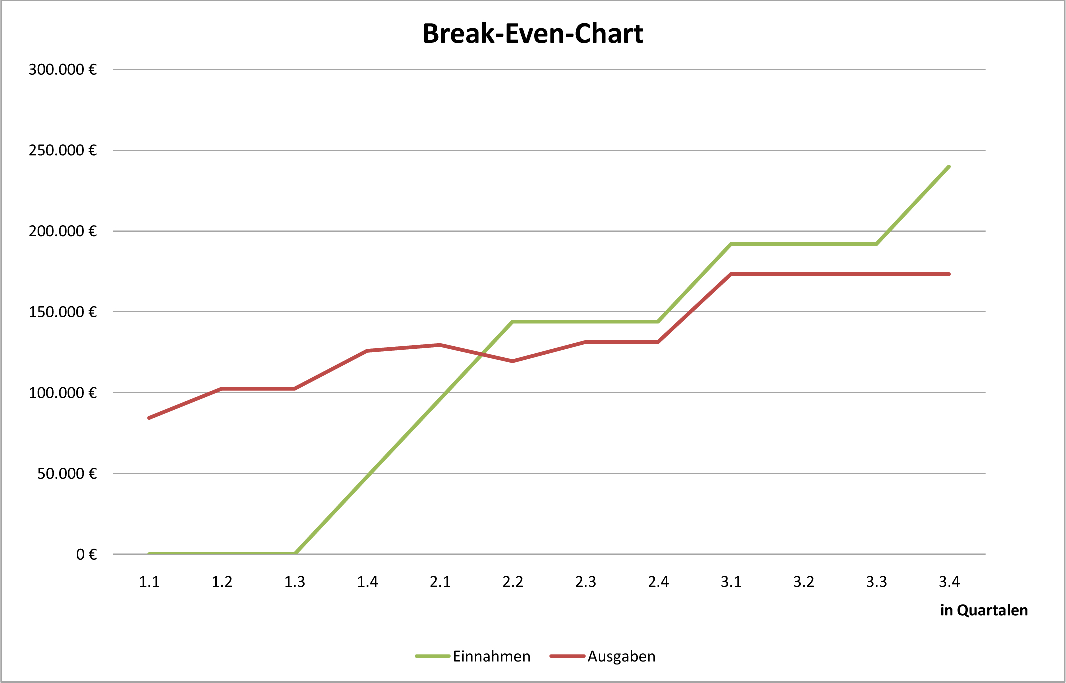
\includegraphics[width=0.8\linewidth]{../Bilder/BreakEvenChart}
\caption{Break-Even-Chart unseres Finanzplans}
\label{fig:BreakEvenChart}
\end{figure}
